% !TeX root = ../tesis.tex

\chapter{Antecedentes y Marco Teórico}
\label{ch:marco-teorico}

Al inicio del siglo XX, la capital mexicana contaba con escasos tranvías eléctricos
y unos pocos transportes de ruta, pero a medida que avanzó el siglo, la población
también creció, lo que obligó al gobierno federal a invertir en los transportes
colectivos. Este avance se vio frenado con el estallido de la Revolución Mexicana
en 1910, movimiento que no cesó hasta mediados de 1930. Para esos años ya se
habían implementado nuevas rutas de transporte colectivo, como la creación del
naciente tranvía y sus rutas que partían del centro de la Ciudad. Otro avance
notorio fue la promulgación de nuevos transportes de ruta a localidades alejadas,
siendo estos mayormente camiones. Sin embargo, el interés por la expansión de las
áreas urbanas no se dio hasta la época llamada ``El Milagro Mexicano'', la cual
abarca desde los inicios de 1940 hasta mediados de la década de 1970, según
\textcite{molina2018}.

Es a partir del Cardenismo que la reconstrucción de la economía, la infraestructura
y el tejido político se consumó, haciendo necesaria una inversión significativa sobre
las ciudades y su comunicación. En su informe entregado ante las cámaras federales
de 1935, el Ejecutivo reportó una recuperación notoria en las arcas públicas,
destinando buena parte del cálculo presupuestal a las necesidades sociales y de
comunicación:

\begin{quote}
``Es verdaderamente satisfactorio para el Encargado del Poder Ejecutivo de la
Nación dirigirse a sus conciudadanos con motivo del primero de año, enviándoles un
mensaje cordial y lleno de optimismo, pues las condiciones del país nos permiten
afirmar que algunos de los anhelos trascendentales del pueblo podrán realizarse
totalmente en el presente ciclo, e iniciarse la ejecución de otros varios que
complementen la base de un período nuevo de positivo progreso.''
\parencite[pp.~2--4]{biblioteca1935}
\end{quote}

Con este contexto, el urbanismo experimentó un acelerado crecimiento, el mismo
que se empalma con las necesidades de un país que transitaba de los caudillos y lo
rural hacia lo institucional y urbano.

% -----------------------------------------------------------------------
\section{La Hegemonía del Automóvil y la adopción de la automovilidad}
\label{sec:hegemonia-automovil}
% -----------------------------------------------------------------------

El problema de movilidad que actualmente afecta a la \cdmx{} y su periferia no es
un fenómeno coyuntural, sino el resultado de una adopción histórica y cultural de la
automovilidad como paradigma urbano. Este concepto, definido por
\textcite{franco2022} en su tesis sobre el periodo 1903--1933, establece que el
vehículo privado dejó de ser un simple medio de transporte para convertirse en el
eje estructurador de la política pública y el imaginario social.

Esta adopción se consolidó a mediados del siglo XX con la priorización política de
la infraestructura vial sobre otros modos de transporte. El crecimiento vehicular en
el Distrito Federal fue exponencial, pasando de 150,584 unidades en 1955 a
209,904 en 1958 \parencite{perlo2023}, una demanda que el Estado decidió gestionar
no mediante la diversificación modal, sino a través de la expansión de la red de
carreteras urbanas, sellando así la dependencia estructural al automóvil que
caracteriza la problemática actual.

% -----------------------------------------------------------------------
\section{El Anillo Periférico: Un Proyecto Político Estructural}
\label{sec:anillo-periferico}
% -----------------------------------------------------------------------

La construcción del Anillo Periférico, junto con el Viaducto Miguel Alemán, debe
analizarse no como una simple necesidad de infraestructura, sino como la expresión
material y simbólica de la hegemonía de la automovilidad como política de Estado
durante la regencia de Ernesto P. Uruchurtu (1952--1966) \parencite{franco2022}.
La magnitud de estas obras subraya el giro drástico que la administración de Ruiz
Cortines imprimió a la agenda de gobierno para el Distrito Federal, requiriendo un
funcionario con la energía y la afinidad ideológica de Uruchurtu, cuya trayectoria
previa le había proporcionado un conocimiento directo de la función administrativa
del \textsc{ddf} \parencite[Tomo~1, p.~173]{perlo2023}.

% -----------------------------------------------------------------------
\subsection{Centralización Administrativa y la Creación de los XII Cuarteles}
\label{subsec:xii-cuarteles}
% -----------------------------------------------------------------------

Antes de la ejecución de la mega-obra vial, la regencia de Uruchurtu se enfocó en
la reestructuración administrativa y financiera del Departamento del Distrito Federal
(\textsc{ddf}). Esta etapa inicial (1952--1953) incluyó una reforma a la recaudación
de impuestos que generó un aumento sustancial del presupuesto para obra pública,
lo cual sentó las bases para el posterior desarrollo urbano.

Derivado de este crecimiento poblacional y la necesidad de optimizar la prestación
de servicios, el regente procedió a la división del \textsc{ddf} en doce Cuarteles.
Según la documentación, esta delimitación fue estrictamente administrativa y de
vigilancia, sin peso político-estatal directo, orientada a un control poblacional y
estratégico de la Ciudad de México. No obstante, el alcance de esta estrategia fue
rápidamente superado por la expansión física de la mancha urbana que forjó la
naciente Área Metropolitana de la Ciudad de México.

La importancia de esta división radica en su impacto urbanístico posterior: el diseño
del Anillo Periférico y el Circuito Interior representó la materialización geográfica
de los límites de estos Cuarteles \parencite[Tomo~1, p.~257]{perlo2023}. Esta
correlación entre el límite administrativo de control y la infraestructura vial más
ambiciosa de la época permite afirmar que la creación de ambos circuitos fungió como
una delimitación operativa y simbólica que, si bien fue superada en su función de
control, sigue siendo una referencia fundamental en la división económica y política
de la capital.

\begin{figure}[H]
    \centering
    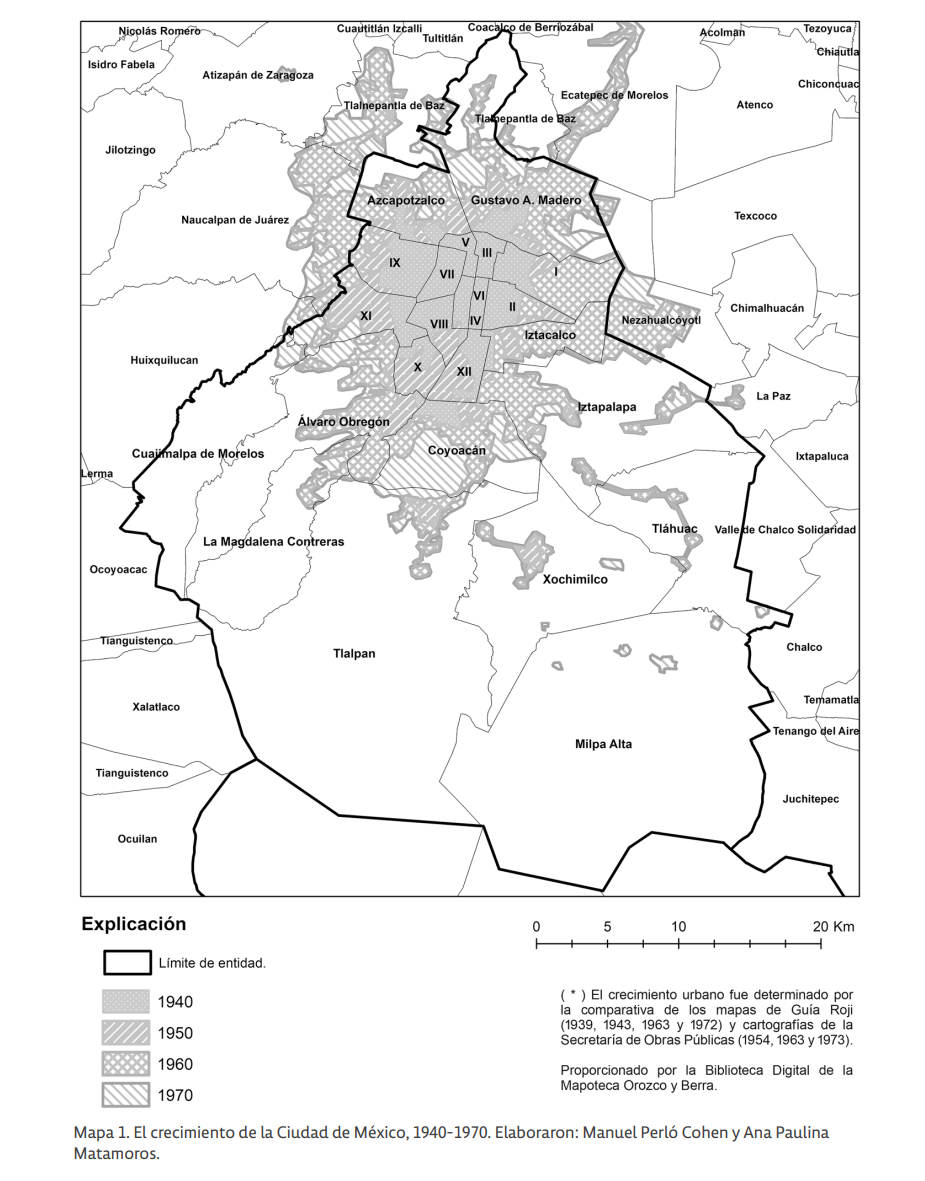
\includegraphics[width=0.82\textwidth]{Figures/Cap1/Uruchurtu1}
    \caption[Designación de los XII Cuarteles en la Ciudad de México]{Designación
    de los XII Cuarteles en la Ciudad de México y crecimiento de la mancha urbana
    (1940--1970).}
    \label{fig:xii-cuarteles}
    \fuentefigura{Perlo Cohen (2023, p.~257).}
\end{figure}

% -----------------------------------------------------------------------
\subsection{La Prioridad Presupuestal: El Sesgo Vial Hegemónico}
\label{subsec:sesgo-vial}
% -----------------------------------------------------------------------

La materialización de la modernidad urbana, bajo la óptica de Uruchurtu, se basó en
la implementación de grandes avenidas y vías rápidas orientadas exclusivamente al
automóvil. Entre las obras más destacadas se encuentran el Viaducto Miguel Alemán,
la Avenida Río Churubusco, el Circuito Interior y el Anillo Periférico. Este último,
que se extendía desde Cuatro Caminos hasta Cuemanco, se concibió como la
principal arteria de comunicación, representando una obra moderna y cosmopolita
destinada a servir al flujo vehicular masivo.

La decisión de priorizar estas obras no fue una casualidad de la planeación, sino un
sesgo presupuestal deliberado. \textcite[Tomo~1, p.~391]{perlo2023} documenta que
solo en 1958, el \textsc{ddf} destinó \$408 millones de pesos a obras en avenidas,
banquetas, pavimentos y pasos a desnivel. Esta inversión superó con creces la suma
destinada a servicios sociales esenciales como mercados, escuelas y centros
asistenciales, evidenciando que la eficiencia del flujo vehicular era el criterio rector
del desarrollo urbano por encima de la equidad social o la integración territorial.

% -----------------------------------------------------------------------
\subsection{El Déficit Estructural y el Rechazo al Metro}
\label{subsec:rechazo-metro}
% -----------------------------------------------------------------------

A pesar de la magnitud de la inversión vial, el \textsc{ddf} afrontaba una crisis de
movilidad imposible de ignorar. Para finales de la década de 1950, la mayoría de la
población carecía de automóvil propio, dependiendo de un sistema de autobuses de
rutas concesionadas caracterizado por ser precario e ineficiente. La respuesta del
gobierno se limitó a la ampliación de rutas y a la promoción de transportes eléctricos
(trolebuses y tranvías), una estrategia insuficiente ante el crecimiento desmedido
de la urbe.

El punto de inflexión que definió el futuro de la movilidad capitalina fue el rechazo
de Uruchurtu a la propuesta de un tren subterráneo ---el actual Sistema de Transporte
Colectivo Metro---, presentada por el ingeniero Bernardo Quintana Arrioja a principios
de la década de 1960. El regente desestimó la idea por considerarla costosa,
invasiva e innecesaria, argumentando la supuesta inviabilidad del proyecto debido al
suelo fangoso de la ciudad. Esta decisión tuvo un impacto trascendental, retrasando
la construcción del Metro hasta 1967 y consolidando el predominio del transporte
superficial y motorizado.

En síntesis, las obras de Uruchurtu carecieron de un programa articulado y basado
en un patrón urbanístico refinado, respondiendo principalmente a las necesidades
inmediatas que el regente logró identificar. El legado del Periférico es una
fragmentación funcional: internamente, delimitó el orden administrativo de los XII
Cuarteles; externamente, propició un crecimiento sin orden que ha dejado a los
territorios periféricos sin conectividad de transporte masivo hasta el día de hoy.

% -----------------------------------------------------------------------
\section{Marco Teórico: Dispersión, Fragmentación y Equidad}
\label{sec:marco-teorico-dispersion}
% -----------------------------------------------------------------------

La consecuencia directa del modelo vial radial fue la expansión desordenada de la
mancha urbana en un proceso denominado \termino{dispersión}. Sin embargo, para
los fines de esta tesis, el concepto más relevante es la \termino{fragmentación
urbana}, ya que denota una ruptura funcional y social que va más allá de la simple
extensión física del territorio.

\textcite{padilla2007} argumenta que la fragmentación se manifiesta en una dislocación
de la cohesión urbana y social, donde las nuevas áreas periféricas carecen de una
adecuada conexión funcional con el centro y entre sí. Esta dislocación se traduce en
una desigualdad de acceso que perpetúa las brechas socioespaciales. Por lo tanto,
el problema a resolver en el Anillo Periférico es la fragmentación territorial resultante
del modelo radial, que impide la movilidad equitativa para las alcaldías del sur.

% -----------------------------------------------------------------------
\subsection{Limitaciones del Modelo Radial}
\label{subsec:limitaciones-radial}
% -----------------------------------------------------------------------

La planificación del transporte público en la \cdmx{} siguió el esquema descrito por
\textcite{molinero2002}, donde las rutas radiales se priorizan para conectar áreas
periféricas con un Distrito Central de Negocios (\textsc{cbd}, por sus siglas en
inglés). Este esquema predominó durante la segunda mitad del siglo XX, cuando la
ciudad experimentó un crecimiento urbano desmedido. Sin embargo, en ciudades
con más de 300,000 habitantes este tipo de rutas comienza a ser ineficiente, ya que
concentra los movimientos en el centro y no considera las necesidades de
desplazamiento entre otras áreas urbanas \parencite{molinero2002}.

% -----------------------------------------------------------------------
\subsection{Transiciones de Fase en Redes Urbanas}
\label{subsec:transiciones-fase}
% -----------------------------------------------------------------------

A la fecha de realización de este estudio (2025), no existe en la \cdmx{} alguna ruta
circular que sirva de soporte para el transporte público masivo colectivo. A pesar de
que la Ciudad cuenta con una vialidad de trazo circular (el Anillo Periférico), ésta
se ha orientado históricamente al automóvil privado. Esta ausencia representa una
\termino{brecha topológica} en la red: la inexistencia de conexiones transversales
impide que el sistema alcance una mayor eficiencia ante el crecimiento continuo de
la demanda.

% -----------------------------------------------------------------------
\subsection{Minimización de Transferencias en Redes Anillo-Radiales}
\label{subsec:minimizacion-transferencias}
% -----------------------------------------------------------------------

Desde la perspectiva de la teoría de redes, \textcite{owais2020} demuestra que la
incorporación de una geometría anillar a un sistema predominantemente radial reduce
el número de transbordos necesarios para conectar zonas periféricas entre sí. Esta
minimización de transferencias no solo mejora los tiempos de traslado, sino que
incrementa la percepción de calidad del servicio por parte del usuario, al reducir la
fricción del viaje multimodal que caracteriza actualmente la movilidad en las alcaldías
del sur de la \cdmx{}.

% -----------------------------------------------------------------------
\section{Teoría Latinoamericana}
\label{sec:teoria-latinoamericana}
% -----------------------------------------------------------------------

Para enmarcar el caso de la \cdmx{} en un contexto de crítica urbanística regional,
es fundamental recurrir a la teoría sobre la ciudad en América Latina. La obra
compilatoria de \textcite{padilla2007} proporciona el marco conceptual para entender
que la crisis de movilidad en la periferia es síntoma de un agotamiento del modelo
de planeación estatal y la adopción de enfoques que favorecieron el capital
inmobiliario y la privatización del espacio. La incapacidad de la planeación urbana
para gestionar la expansión territorial generada por los grandes proyectos viales,
como el Periférico, es el caldo de cultivo para la emergencia de la ciudad neoliberal.

La propuesta de un corredor circular es, en este contexto teórico, un esfuerzo por
revertir el impacto de la automovilidad hegemónica y la planificación fragmentada.
Busca pasar de un enfoque que prioriza la velocidad del flujo ---propio de la era
Uruchurtu--- a uno que prioriza la integración equitativa y la eficiencia operativa,
alineado con las demandas de un nuevo modelo de ciudad que ya no puede ser
definido únicamente por sus arterias motorizadas \parencite{franco2022}.

% -----------------------------------------------------------------------
\section{Casos Similares en Otros Países}
\label{sec:casos-similares}
% -----------------------------------------------------------------------

La implementación de corredores circulares de transporte masivo no es una idea
nueva a nivel global. Su efectividad ha sido documentada en diversas megaciudades
que enfrentaban problemas estructurales similares a los de la \cdmx{}: redes
radiales saturadas, periferias desconectadas y tiempos de traslado crecientes.

El caso más representativo es la \textbf{Gran Línea Circular del Metro de Moscú},
inaugurada en 2023 con 70 kilómetros de longitud. Esta línea fue concebida
explícitamente para descomprimir las líneas radiales del centro y articular la
movilidad entre zonas periféricas sin necesidad de pasar por las estaciones
centrales más congestionadas \parencite{efe2023}. Su puesta en operación
demostró cómo la adopción de geometrías anillares puede cambiar cualitativamente
la eficiencia de todo el sistema de transporte de una capital.

Un segundo referente es el \textbf{\textit{Suburban Rail Loop} de Melbourne},
Australia, actualmente en planeación y construcción. Este proyecto parte de un
diagnóstico análogo al de la \cdmx{}: las alcaldías del llamado \textit{Middle-Ring}
albergan hospitales, universidades y centros de empleo de alta demanda, pero
carecen de una conectividad lateral robusta que los articule entre sí
\parencite{suburbanrailloop2021}. El proyecto busca transformar una serie de
suburbios desconectados en una red policéntrica de precintos de innovación y
empleo, mediante la inserción de un corredor ferroviario de arco periférico.

Estos referentes internacionales validan la hipótesis central de esta investigación:
la inserción de una ruta anillar en la sección sur del Periférico no es una solución
experimental, sino una estrategia probada y replicable en el contexto específico de
la \cdmx{} y su \zmvm{}.